\documentclass[11pt]{article}
\usepackage{times}
\usepackage{array}
\usepackage{longtable}
\usepackage{booktabs}
\usepackage{amssymb}
\usepackage{marvosym}
\usepackage{wasysym}
\usepackage{tabularx}
\usepackage{pifont}
\usepackage{color}
\usepackage{listings}
\usepackage[pdftex]{graphicx}    % Zur Einbindung von PDF-Bildern
\usepackage{float}
% \usepackage{floatflt}
\usepackage{wrapfig}
\usepackage[margin=10pt,justification=centering, font=small,labelfont=bf,labelsep=newline,format=plain,singlelinecheck=off]{caption}


%Kopfzeile
\pagestyle{headings}
% Ende Kopfzeile

\DeclareGraphicsExtensions{.png} % Dateiendung fuer PDF-Bilder
\graphicspath{{./images/}}        % Festlegung des Pfades zu den Bildern
\usepackage{upquote}
%\usepackage{pictex}
\usepackage[T1]{fontenc}
\usepackage {hyperref}
%\usepackage{german}
\usepackage [latin1] {inputenc}
%\usepackage[babel,german=quotes]{csquotes} % Deutsche
%\usepackage[german]{babel}
\usepackage{alltt}

%\usepackage{mathptmx,times} \renewcommand{\fett}{\vec}
%

\parindent 0pt %ruecke Absatzbeginn nicht ein wenn neuer Absatz beginnt

%\lstset{numbers=left, numberstyle=\tiny, numbersep=-5pt,commentstyle=\color{hellgrau},  backgroundcolor=\color{white},xleftmargin=10pt, breaklines=true, breakautoindent=true,basicstyle=\ttfamily\footnotesize,showspaces=false, }
\lstset{numbers=none, numberstyle=\tiny, numbersep=-5pt,commentstyle=\color{hellgrau},  backgroundcolor=\color{white},xleftmargin=10pt, breaklines=true, breakautoindent=true,basicstyle=\ttfamily\footnotesize,showspaces=false, }
\lstset{language={[Visual]Basic}, showstringspaces=false}
\lstset{emph={function }, emphstyle=\color{blue}, tabsize=10,framexleftmargin=0mm, frame=shadowbox, rulesepcolor=\color{hellgrau}, frameround=tttt, prebreak = {\ding{229}}}



\topmargin0mm
\textheight230mm
\textwidth170mm
\oddsidemargin2mm
\evensidemargin-12mm




\renewcommand{\topfraction}{0.85}
\renewcommand{\textfraction}{0.1}
\setcounter{totalnumber}{8}
\setcounter{topnumber}{8}
\setcounter{bottomnumber}{8}
\pagestyle{headings}

\begin{document}

\section*{Klausur 28.01.2015}
\vspace{30pt}
\textbf{Erstellen Sie zun�chst im Verzeichnis iksy05 ein Verzeichnis, dem Sie Ihren Namen geben. In diesem Verzeichnis speichern Sie alle Dateien Ihrer L�sung. Dateien, die sich nicht in diesem Verzeichnis befinden, werden nicht gewertet.}

Sie sind Mitarbeiter der neu gegr�ndeten Nationale Salzreserve, die f�r die Kommunen in Deutschland Streusalz bereitstellt. Sie sollen ein Programm schreiben, mit dem die Salzkosten f�r die Kommunen berechnet werden k�nnen. 

Die Berechnung basiert auf der L�nge der zu streuenden Stra�en und den erwarteten Einsatztagen. Je Kilometer Stra�enl�nge werden je Einsatztag 70 kg Salz kalkuliert. Ein Teil dieser Stra�en sind Nebenstra�en. F�r diese werden 30\% weniger Salz gerechnet. Eine Tonne Salz kostet zurzeit 180 Euro.

Die ``Nationale Salzreserve'' gibt Rabatt: 10\% bei Bestellungen ab 700 Tonnen, 20\% bei Bestellungen ab 1000 Tonnen Salz.

�bersteigt der Preis 100000 Euro, wird ein zus�tzlicher Rabatt von 10 Prozent gegeben.
Hinweis: 1 Tonne entspricht 1000kg.

Die erwarteten Einsatztage sind von der Stadt abh�ngig. Sie k�nnen sie aus der Tabelle Kommune in der Datenbank wiInf\_Streusalz ermitteln. Die Datenbank befindet sich auf Ihrem lokalen Rechner (Adresse 127.0.0.1) Benutzername und Passwort sind jeweils wiInf. Die Tabelle Kommune hat folgende Struktur:

%---Figure:-------------------------------------------
\begin{figure}[htb]
        \begin{center}
	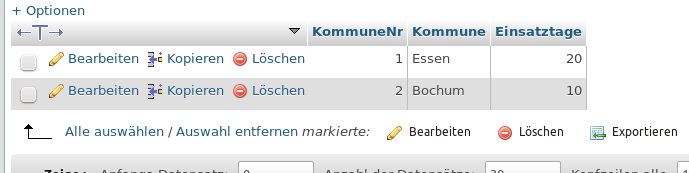
\includegraphics[width=14cm]{./produkt.png}
	\caption{\label{Tabelle1} \textsl{Tabelle Kommune}}
  \end{center}
\end{figure}
%-----------------------------------------------------

Die Datenbankfunktionen werden in der Klasse DbFunctions gekapselt, f�r den Zugriff auf die Tabellen erstellen sie eine Klasse Kommune, in der die Zugriffsfunktionen oder die Zugriffsfunktion gespeichert werden. Die Berechnung des Ergebnisses lagern Sie in eine eigene Klasse aus.


F�hren Sie alle aus Sicherheitsgr�nden notwendigen Pr�fungen durch, auch bei den Eingaben, die nicht direkt f�r den Datenbankzugriff genutzt werden. 

Stellen Sie weiterhin folgendes client-seitig bereits sicher:
\begin{itemize}
\item Die L�nge des Stra�ennetzes und die L�nge der Nebenstra�en m�ssen positive Zahlen sein.
\item Die L�nge des Stra�ennetzes muss zwischen 1000 und 10000 liegen.
\item Alle Eingaben sind erforderlich.
\end{itemize}
Pr�fen Sie diese Validit�ten auch auf dem Server, und verhindern Sie die Ausf�hrung des Skripts bei unerlaubten Eingaben.

Die Darstellung erfolgt �ber die Klassenbibliothek Smarty, die client-seitigen Eingabekontrollen �ber HTML 5.

Einen Screenshot einer Eingabeseite mit zugeh�riger Ausgabe sehen Sie hier:
%---Figure:-------------------------------------------
\begin{figure}[htb]
        \begin{center}
	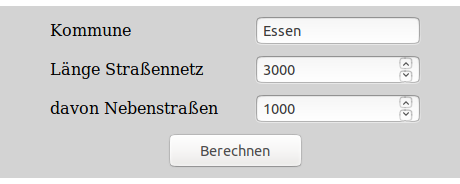
\includegraphics[width=10cm]{./eingabe}
	\caption{\label{Eingabeseite} \textsl{Eingabeformular}}
  \end{center}
\end{figure}
%-----------------------------------------------------
\linebreak[2]

%---Figure:-------------------------------------------
\begin{figure}[htb]
        \begin{center}
	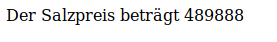
\includegraphics[width=6cm]{./ausgabe}
	\caption{\label{Eingabeseite} \textsl{Ausgabe}}
  \end{center}
\end{figure}
%-----------------------------------------------------

\end{document}
